% Commented out: 
% \addbibresource
% \includepdf

\documentclass[12pt,letterpaper,english,bibliography=totocnumbered, abstract=on]{scrartcl}

\usepackage{indentfirst}
\usepackage[titletoc]{appendix}
\usepackage{fullpage}
%\usepackage{subfiles}
\usepackage[T1]{fontenc}
\usepackage[latin9]{inputenc}
\usepackage{color}
\usepackage{babel}
\usepackage{verbatim}
\usepackage[unicode=true,pdfusetitle,
bookmarks=true,bookmarksnumbered=false,bookmarksopen=false,
breaklinks=true,pdfborder={0 0 0},pdfborderstyle={},backref=false,colorlinks=true]
{hyperref}
\hypersetup{linkcolor=blue,citecolor=blue,urlcolor=blue}

\usepackage{booktabs}
\usepackage{multirow}
\usepackage{adjustbox}
\usepackage{threeparttable}
\usepackage[table]{xcolor}
\usepackage{csquotes}
\usepackage{soul} % for hiliting text: \hl

\usepackage[backend=biber, style=authoryear, maxbibnames=99, dashed=false]{biblatex}
\setlength\bibitemsep{2\itemsep}
%\addbibresource{mylibrary.bib}
%\addbibresource{CRB.bib}

\usepackage{pdfpages}
\usepackage{float} % Allows use of H to place floats

\usepackage{pgfgantt}

\usepackage{framed}

\usepackage{graphicx}

% Prevent page breaks within paragraphs
% https://tex.stackexchange.com/questions/21983/how-to-avoid-page-breaks-inside-paragraphs
\widowpenalties 1 10000

\begin{document}

\titlehead{TECHNICAL REPORT}

\title{Larval Diet Experiment}

\author{Jim Grasela, Chris Cayanan, and Aubrey Moore\\University of Guam}

\maketitle
%\footnote{\url{https://github.com/aubreymoore/2020-FS-CRB-biocontrol-project/blob/master/combined-proposal.pdf}}
\newpage
\tableofcontents

\pagebreak

\section{Background}

\section{Methods}

\newpage
\section{Results}

\subsection{Egg survival}

\begin{figure}[H]
	\centering
	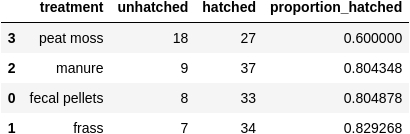
\includegraphics[width=0.6\linewidth]{egg_survival_table.png}
	\caption{Egg survival.}
	\label{fig:eggsurvivaltable}
\end{figure}

\begin{figure}[H]
	\centering
	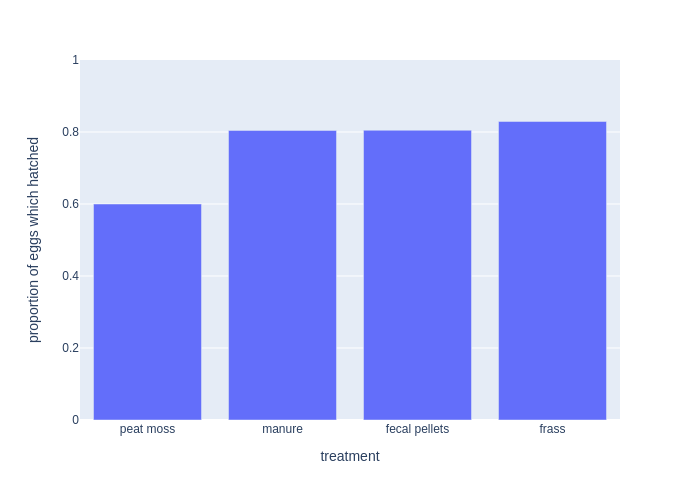
\includegraphics[width=0.6\linewidth]{egg_survival_plot}
	\caption{Egg survival. Chi2 result of the contingency table: 8.2706, p-value: 0.0407.
	Post-hoc tests did not indicate any pair-wise differences.}
	\label{fig:eggsurvivalplot}
\end{figure}

\begin{footnotesize}
	\begin{verbatim}
		Chi2 result of the contingency table: 8.270648694989156, p-value: 0.04073715987248983
		
		Post-hoc chi2 tests results:
		('fecal pellets', 'frass'): p_value: 1.000000; corrected: 1.000000 (ns) reject: False
		('fecal pellets', 'manure'): p_value: 0.791311; corrected: 1.000000 (ns) reject: False
		('fecal pellets', 'peat moss'): p_value: 0.067072; corrected: 0.134144 (ns) reject: False
		('frass', 'manure'): p_value: 0.982206; corrected: 1.000000 (ns) reject: False
		('frass', 'peat moss'): p_value: 0.035652; corrected: 0.134144 (*) reject: False
		('manure', 'peat moss'): p_value: 0.056902; corrected: 0.134144 (ns) reject: False
	\end{verbatim}
\end{footnotesize}

\subsection{Larval survival}

\begin{figure}[H]
	\centering
	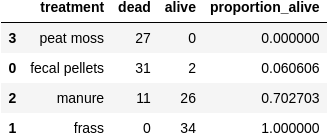
\includegraphics[width=0.7\linewidth]{larval_survival_table}
	\caption{Larval survival.}
	\label{fig:larvalsurvivaltable}
\end{figure}

\begin{figure}[H]
	\centering
	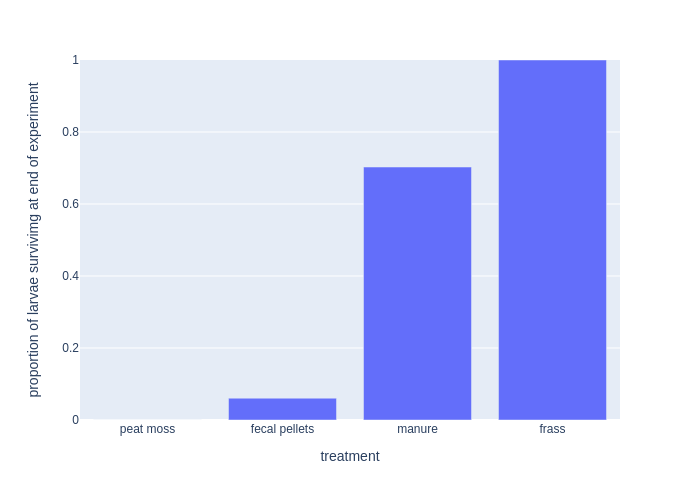
\includegraphics[width=0.7\linewidth]{larval_survival_plot}
	\caption{Larval survival.}
	\label{fig:larvalsurvivalplot}
\end{figure}

\begin{footnotesize}

\begin{verbatim}
Chi2 result of the contingency table: 92.45587408140003, p-value: 6.501188043511334e-20

Post-hoc chi2 tests results:
('fecal pellets', 'frass'): p_value: 0.000000; corrected: 0.000000 (****) reject: True
('fecal pellets', 'manure'): p_value: 0.000000; corrected: 0.000000 (****) reject: True
('fecal pellets', 'peat moss'): p_value: 0.563092; corrected: 0.563092 (ns) reject: False
('frass', 'manure'): p_value: 0.001747; corrected: 0.002096 (**) reject: True
('frass', 'peat moss'): p_value: 0.000000; corrected: 0.000000 (****) reject: True
('manure', 'peat moss'): p_value: 0.000000; corrected: 0.000000 (****) reject: True
\end{verbatim}

\end{footnotesize}

\subsection{Larval mass}

\begin{figure}[H]
	\centering
	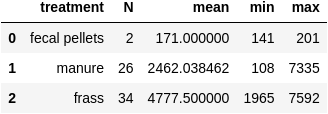
\includegraphics[width=0.7\linewidth]{larval_mass_table}
	\caption{Larval mass.}
	\label{fig:larvalmasstable}
\end{figure}

\begin{figure}[H]
	\centering
	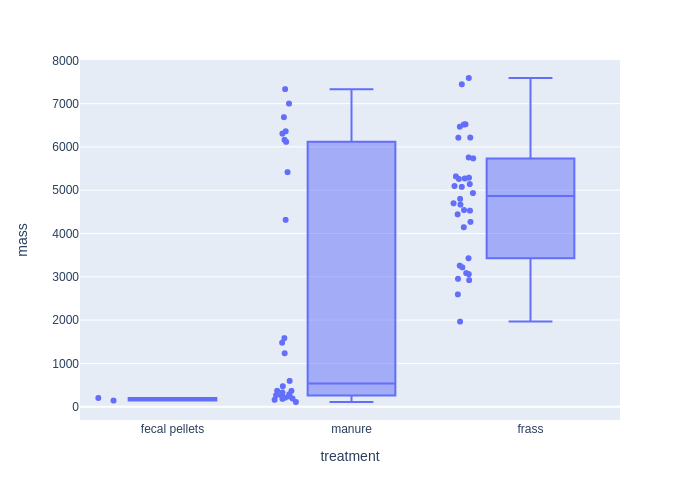
\includegraphics[width=0.7\linewidth]{larval_mass_plot}
	\caption{Larval mass.}
	\label{fig:larvalmassplot}
\end{figure}


\end{document}
